%%%%%%%%%%%%%%%%%%%%%%%%%%%%%%% TO DOS %%%%%%%%%%%%%%%%%%%%%%%%%%%%%%%
% 1. 
%%%%%%%%%%%%%%%%%%%%%%%%%%%%%%%%%%%%%%%%%%%%%%%%%%%%%%%%%%%%%%%%%%%%%%

\section{Introduction} 
\label{sec:intro}
%%%%%%%%%%%%%%%%%%%%%%%%%%%%%%%%% DCC is here %%%%%%%%%%%%%%%%%%%%%%%%%%%%%%%%%%
Today's datacenters (DCs) are server-centric: users rent servers with
specific hardware capabilities tailored to their needs (e.g.,
compute-intensive EC2 instances from Amazon). 
A \emph{disaggregated} datacenter (DDC) disaggregates, or separates,
the resources in a traditional DC into resource \emph{blades},
with each resource connected directly to an interconnect (Figure~\ref{fig:DDC}). 
We use the term \emph{blade} to describe a 1U server containing one resource
type, and \emph{resource} for an individual CPU, DIMM, SSD, etc. in a blade. 

%%%%%%%%%%%%%%%%%%%%%%%%%%%%%%%%% DDC benefits %%%%%%%%%%%%%%%%%%%%%%%%%%%%%%%%%

The modularity of DDCs benefits both operators and
users~\cite{Han2013}. By separating resources into blades, a
DDC provides efficiency: the operator can upgrade specific hardware
blades without impacting other resources types. Users also experience
an efficiency win: in a DDC a user can provision the exact amount of
resources they require and dynamically expand/shrink this set. This flexibility
also increases the DC resource utilization.

%%%%%%%%%%%%%%%%%%%%%%%%%%%%% Research challenges %%%%%%%%%%%%%%%%%%%%%%%%%%%%%%

There are two broad types of disaggregation: partial and full.
In partial disaggregation compute resources have a small amount of
local memory,
memory and storage resources have CPUs,
and a NIC is attached to each resource. 
In full disaggregation each resource is independent and is directly
connected to the rack interconnect. Current research focuses on the practicality
of partial disaggregation~\cite{IntelRSA,Gao2016,Lim2009,Lim2012}.

In this paper, we discuss partial disaggregation at rack-scale:
resources can only connect to other resources in the same rack (e.g., a CPU in
rack1 cannot connect to a DIMM in rack2).
The disaggregated rack is presented to the
client as a single machine through a virtualization layer. Applications can
request a number of VMs to allocate among the racks.
Distributed applications might then run among several disaggregated racks, while
a single-machine application will reside in one rack.


%%%%%%%%%%%%%%%%%%%%%%%%%%%%%%%%%%%%%%%%%%%%%%%%%%%%%%%%%%%%%%%%%%%%%%%%%%%%%%%%
\begin{figure}
    \centering
    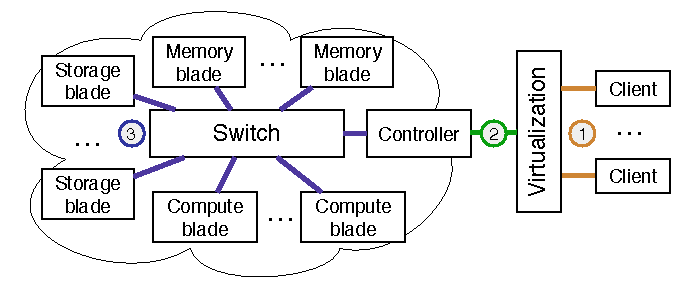
\includegraphics[width=\columnwidth]{fig/ddc-overview}
    \caption{Simplified representation of a disaggregated datacenter with
    three communication points: (1) between the application and the
    virtualization layer,
    (2) between the virtualization layer and the physical resources, and (3)
    between the physical resources bundled as blades.}
    \label{fig:DDC}
\end{figure}
%%%%%%%%%%%%%%%%%%%%%%%%%%%%%%%%%%%%%%%%%%%%%%%%%%%%%%%%%%%%%%%%%%%%%%%%%%%%%%%%
